\section{Результаты эксперимента и обработка данных}

Схема экспериментальной установки изображена на рис. \ref{experimental_scheme}.
Здесь 1 -- возбуждающий лазер, 2 -- делительная пластина, 3 -- поворотное зеркало,
4, 7 -- объективы, 5 -- образец на медном держателе, 6 -- светофильтр, 8 -- оптоволокно.
Часть лазерного излучения, попадая на делительную пластину, преломляется, проходит
через поворотное зеркало и объективом фокусируется на образец. Свет от образца 
преобразуется объективом в параллельный пучок и проходит обратно через поворотное
зеркало и делительную пластину. Светофильтр пропускает свет, излучённый от образца,
но не пропускает лазерное излучение. Излучение образца фокусируется на оптоволокно,
подключённое к спектрометру. Медный держатель образца опускается в канистру с 
жидким азотом, охлаждая образец. Температура образца измеряется с помощью
термометра. 

\begin{figure}[!h]
    \begin{center}
        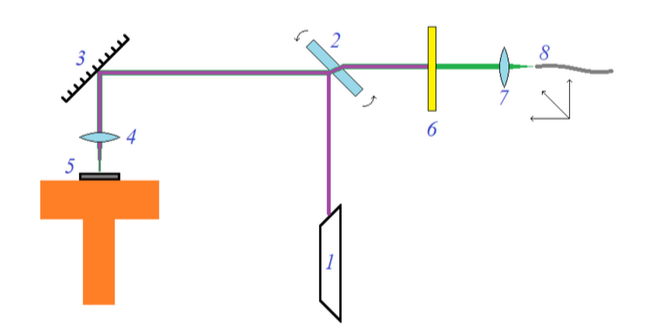
\includegraphics[width=0.7 \linewidth]{experimental_scheme.png}
        \caption{Схема установки}
        \label{experimental_scheme}
    \end{center}
\end{figure}


Результат измерений спектра представлен на рис. \ref{spectre_general}. 
При температурах менее 200 К хорошо видно два пика, соответствующих тонкому 
расщеплению верхнего уровня (левый пик -- переходы C и D, правый пик -- переходы
A и B на рис. \ref{Energy levels}). Ясно, что заселённость верхнего уровня
ниже, чем заселённость нижнего, поэтому левый пик обладает большей интенсивностью.
При температурах более 200 К эти два пика перестают быть различимыми. В любом случае
эти пики (или один пик при больших температурах) аппроксимируется лоренцевским
контуром. Исследуются зависимости ширины профиля на полувысоте и положения максимума
от температуры.  

Основные вклады в погрешность вносят неточность измерения температуры и неточность
измерения длины волны. Во-первых, охлаждение при помощи жидкого азота проводилось
очень быстро, поэтому скорости "обновления показателей" термометра не хватало
для точного определения температуры в данный момент времени. К примеру, показания
термометра могли измениться за "один кадр" на более чем 2 градуса. Во-вторых,
используемый спектрометр измеряет интенсивность с шагом $0.1 \text{ нм}$, а ширина
пика составляет $\sim 1 \text{ нм}$, то есть в исследуемой области находится примерно
30 точек на 2 пика. Последнее обстоятельство усугубляется тем, что слева в спектре 
имеются ещё дополнительные переходы на другие колебательные уровни, которые, конечно,
подавлены по сравнению с основными переходами, но существенно ограничивают область,
в которой есть возможность аппроксимировать пик лоренцианом. Аппроксимация для различных
температур приведена на рис. \ref{approx_lor_contour}. 

\begin{figure}[!h]
    \begin{center}
        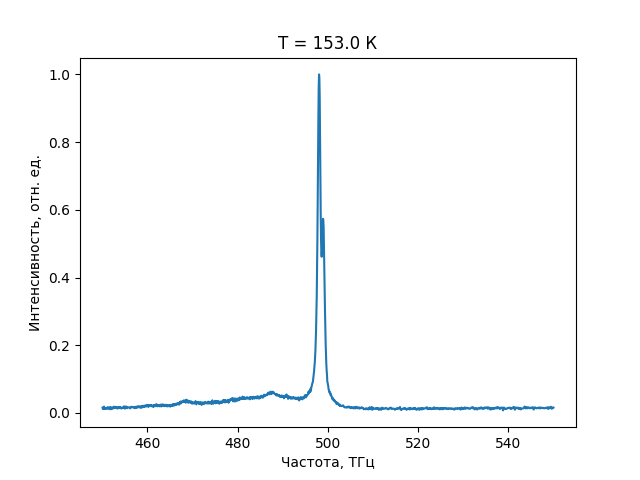
\includegraphics[width=0.7 \linewidth]{spectre_general.png}
        \caption{Спектр люминесценции при температуре T = 153 К.}
        \label{spectre_general}
    \end{center}
\end{figure}


\begin{figure}[!h]
    \begin{minipage}[h]{0.49\linewidth}
        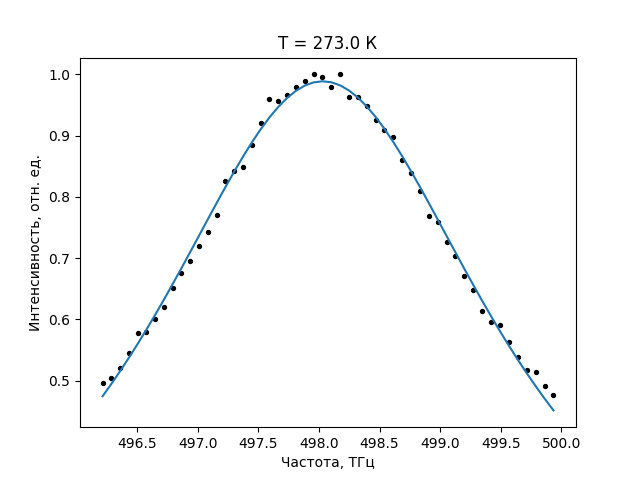
\includegraphics[width = 1.1 \linewidth]{spectre_local_273K.png}
        \\ (a)
    \end{minipage}
    \hfill
    \begin{minipage}[h]{0.49\linewidth}
        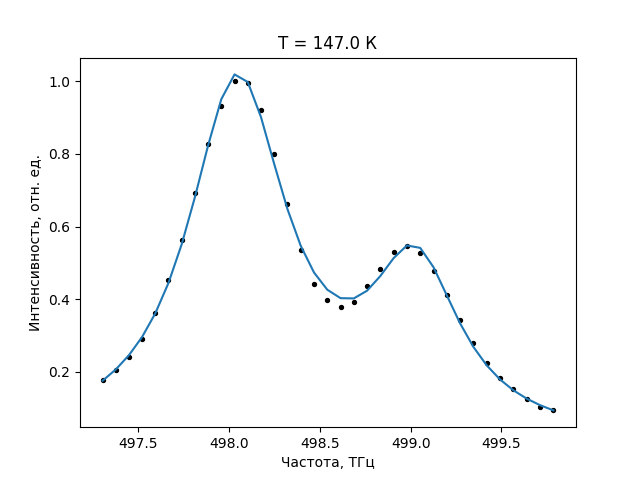
\includegraphics[width = 1.1 \linewidth]{spectre_local_147K.png}
        \\ (b)
    \end{minipage}
    \caption{Аппроксимация лоренцианами пиков спектра люминесценции при температурах
    (a) 273 К, (b) 147 К}
    \label{approx_lor_contour}
\end{figure}


\subsection{Зависимость ширины пика от температуры}
Построим зависимость ширины пика от температуры. Температуры от 210 К до 240 К 
исключены, так как эти температуры являются "переходными" от двух пиков к одному,
аппроксимация в таком случае затруднена. Погрешность измерения температуры оценим в
1 К, погрешность ширины пика -- корень из дисперсии определения параметра ширины пика 
в функции curve\_fit библиотеки scipy, python. Результат приведён на рис. \ref{peak_width}
Зелёная линия -- функция вида $a + bT^3$, приближающая исследуемую зависимость. 
Из графика $a \approx 100 \text{ МГц}$ -- ширина линии при нулевой температуре, что, разумеется,
может соответствовать действительности. При попытке аппроксимировать зависимость
функцией $y \sim \alpha + \beta T^4$ естестественная ширина линии получается в несколько
раз больше, а при функции $y \sim \alpha + \beta T^2$ вообще отрицательной. 
Ясно, что этот приведённый результат соответвует построенной теоретической модели. 

\begin{figure}[!h]
    \begin{center}
        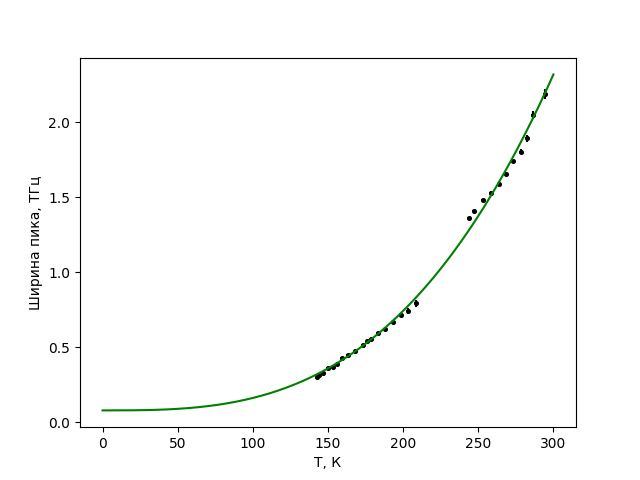
\includegraphics[width=0.9 \linewidth]{peak_width.png}
        \caption{Зависимость ширины пика от температуры}
        \label{peak_width}
    \end{center}
\end{figure}


\subsection{Разность частот тонкого расщепления}
На рис. \ref{delta_frequence} приведён график зависимости величины тонкого
расщепления от температуры с аппроксимацией функцией $\alpha + \beta T^2$ (зелёная
линия). Из графика $\alpha \approx 1.2 \text{ ТГц} \approx 5 \text{ мэВ}$. Видно, что 
при температуре около 200 К ошибка начинает резко возрастать. Связано это с тем, что 
при такой температуре два пика уже перестают быть хорошо различимыми. Таким образом, 
величина тонкого расщепления при 0 К составляет примерно 5 мэВ.


\begin{figure}[!h]
    \begin{center}
        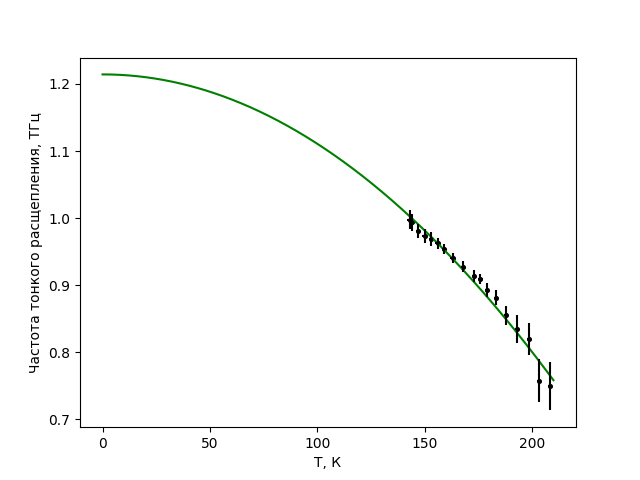
\includegraphics[width=0.9 \linewidth]{delta_frequence.png}
        \caption{Зависимость частоты тонкого расщепления от температуры}
        \label{delta_frequence}
    \end{center}
\end{figure}


\subsection{Длина волны пика}
График зависимости длины волны пика от температуры приведена на рис. 
\ref{mean_peak_wavelenght}. Зелёной линией обозначена аппроксимация 
функцией вида $y = c + dT^3$.


\begin{figure}[!h]
    \begin{center}
        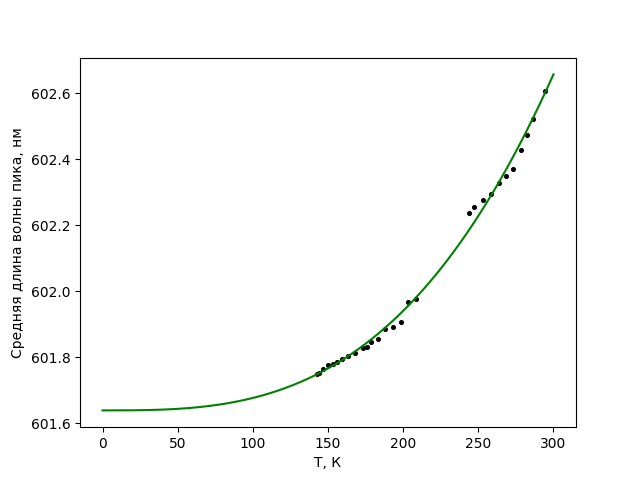
\includegraphics[width=0.9 \linewidth]{mean_peak_wavelenght.png}
        \caption{Зависимость длины волны пика от температуры}
        \label{mean_peak_wavelenght}
    \end{center}
\end{figure}



